\documentclass[article,10pt]{llncs}
\usepackage{makeidx}  % allows for indexgeneration

\usepackage[latin1]{inputenc}
%\usepackage[francais]{babel}
\usepackage{subfigure}
\usepackage{graphicx}
\usepackage{graphics}
\usepackage{dsfont}
\usepackage{natbib}
\usepackage{amsfonts,amsmath,amssymb}
\usepackage{enumerate}
\usepackage{stmaryrd}
\usepackage{color}
\usepackage{ulem}
\usepackage{float}
\floatstyle{ruled}
\usepackage{algpseudocode}
\usepackage{algorithmicx}
\usepackage{algorithm}
\usepackage{url}
\usepackage[table]{xcolor}

%\newfloat{Algorithm}{thp}{lop}
%\floatname{Algorithm}{Algorithm}
%\newtheorem{de}{Definition}[subsection] % les définitions et les théorémes sont
\newtheorem{theo}{Theorem}[section]    % numérotés par section
\newtheorem{lem}[theo]{Lemma}
%\newtheorem{cor}[theo]{Corrolary}
%\newtheorem{prop}[theo]{Proposition}

\newcommand{\soft}{\texttt{cghseg}}
\newcommand{\esoft}{\texttt{cghseg }}


\begin{document}

\title{High Dimension Segmentation using the \texttt{cghseg} package}
%
\titlerunning{High dimension with \texttt{cghseg}}  % abbreviated title (for running head)
%                                     also used for the TOC unless
%                                     \toctitle is used
%
\author{G. Rigaill$^1$, V. Miele$^2$ and F. Picard$^2$}
%
\authorrunning{Rigaill et al.} % abbreviated author list (for running head)
%
%%%% list of authors for the TOC (use if author list has to be modified)
\tocauthor{Guillem Rigaill$^1$, Vincent Miele$^2$, Franck Picard$^2$}
%
\institute{Laboratoire Statistique et G\'{e}nome, UMR CNRS 8071, USC INRA Universit\'{e} d'Evry, F-91037 Evry, France \\
\email{rigaill@evry.inra.fr},\\ 
\and
Laboratoire de Biom\'etrie et Biologie Evolutive, UMR CNRS 5558 Universit\'{e} Lyon 1, F-69622, Villeurbanne, France \\
\email{vincent.miele@univ-lyon1.fr},\\ 
\email{franck.picard@univ-lyon1.fr}
}

\maketitle   

\begin{abstract}
\esoft is fast enough to segment more than 1,000 profiles of length 100,000 in less than ? hours (or less than an afternoon).

\keywords{}
\end{abstract}
\section{Method}

\subsection{Background / Notations}
We consider a signal of length $n$, $\{X_i\}_{i \leq n}$ with $X_i \in \mathbf{R}$.
A segment $r$ is delimited by two change-points and is denoted
 $r = \llbracket t_1, t_2 \rrbracket$.
We define the set of all segmentations of a segment $r$ in $K$ segments as $\mathcal{M}^{(K)}_{(r)} = \mathcal{M}^{(K)}_{t_1, t_2}$.
The $k$-th change of segmentation $m$ in $K$ segments will be denoted by $\tau_k$ with the convention that $\tau_0 = 1$ and $\tau_K = n+1$.
The $k-th$ segment is denoted by $r_k$.
For a given segmentation in $K$ segments we have, $m = \{r_1, r_2 \ldots, r_K\}$ and for all $k \leq K$,  $r_k = \llbracket \tau_k, \tau_{k+1} -1\rrbracket$.

Using the notations of seg-clust (\cite{picard_2007}) the cost of a given segment $r = \llbracket t_1, t_2 \rrbracket$ is given by minus the log-likelihood :
$$ C_{t_1, t_2}^{(1)} =C_{(r)}^{(1)} = -\log\left(\sum_p \pi_p exp\left\{ - \frac{\sum_{i \in r} (x_i - \mu_p)^2 }{ 2 \sigma^2} \right\}\right)$$ 
The optimal cost in $K$ segments from $r = \llbracket t_1, t_2 \rrbracket$ is defined as :
$$C_{t_1, t_2}^{(K)} = C_{(r)}^{(K)} = \min_{m \in \mathcal{M}^{(K)}_{(r)}} \left\{ \sum_{r \in m} C^{(1)}_{(r)} \right\}.$$
The corresponding  optimal segmentation is defined as :
$$\widehat{m}_{t_1, t_2}^{(K)} = \widehat{m}_{(r)}^{(K)} = \underset{m \in \mathcal{M}^{(K)}_{(r)}}{\operatorname{argmin}} \left\{ \sum_{r \in m} C^{(1)}_{(r)} \right\}.$$
The cost or loss of a segmentation is segment additive. Using this segment additivity one can built an $\Theta(Kn^2)$ dynamic programming algorithm to recover the best segmentations (in $1$ to $K$ segments).
 

Here we propose to approximate this loss in a K-mean fashion
More specifically we propose two possible approximations, the first is:
\begin{eqnarray} \widetilde{C}_{(r)}^{(1)} \approx  \min_p \left\{ \sum_{i \in r}\frac{(x_i - \mu_p)^2} {2\sigma^2 }\right\}
\label{equation:approximation2}\end{eqnarray} 
and the second is 
\begin{eqnarray} \widetilde{C}_{(r)}^{(1)} \approx  \min_p \left\{ \sum_{i \in r}\frac{(x_i - \mu_p)^2} {2\sigma^2 } + \log(\pi_p)\right\} .
\label{equation:approximation1}\end{eqnarray} 
In both cases, $\widetilde{C}_{(r)}^{(K)}$ and $\widetilde{m}_{(r)}^{(K)}$ are defined as:
$$ \widetilde{C}_{(r)}^{(K)} =\min_{m \in \mathcal{M}^{(K)}_{(r)}} \left\{ \sum_{r \in m} \widetilde{C}^{(1)}_{(r)} \right\}, \qquad \text{and} \qquad
 \widetilde{m}_{(r)}^{(K)} = \underset{m \in \mathcal{M}^{(K)}_{(r)}}{\operatorname{argmin}} \left\{ \sum_{r \in m} \widetilde{C}^{(1)}_{(r)} \right\}.$$


Importantly using $\widetilde{C}_{(r)}^{(1)}$ rather than  ${C}_{(r)}^{(1)}$ the set of canditate segmentations can be pruned efficently as in \cite{rigaill_2010}. 
In our case given that the set of possible values for $\mu_p$ is finite we can even guarantee the time and space complexity of the algorithm to be $\Theta(KPn)$. 
Furthermore, for the second approximation (given in equation \ref{equation:approximation1}) we can guarantee that the loss of the recovered segmentation $\widetilde{m}_{(r)}^{(K)}$ is at worth within $K \log(p)$ of the optimal segmentation $\widehat{m}_{(r)}^{(K)}$ (see Theorem \ref{theo:theoapprox}).

%%%%%%%%%%%%%%%%%%%%%%%
%%%%%%%%%%%%%%%%%%%%%%%
%%% STD DPA
%%%%%%%%%%%%%%%%%%%%%%%

\subsection{Original dynamic programming algorithm of seg-clust}

The cost of a given segmentation is the sum of the cost of its segments. 
Thus the Bellman optimality principal holds and we have:
$ C_{1, t}^{(k+1)} = min_{\tau \leq t} \{ C_{1, \tau -1}^{(k)}  + C_{\tau, t}^{(1)} \} .$
%More generally for any $k_1 (>0)$ and $k_2 (> 0)$   we have
%$$ C_{1, t}^{(k_1 + k_2)} = min_{\tau \leq t} \{ C_{1, \tau -1}^{(k_1)}  + C_{\tau, t}^{(k_2)} \} $$
Using this update rule  a Dynamic Programming algorithm can be built to recover all $ C_{1, t}^{(k+1)}$ for all $t \leq n$ and $k \leq K$.
This can be done using algorithm \ref{algo:DPA2} for instance. 
For simplicity we did not include the initialization of all $C^{(1)}_{1,t}$ for $t \leq n$ and of all $C^{(k)}_{1,t}$ for $k \leq K$ and $t < k$.
All $C^{(k)}_{1,t}$ are initialized as $+\infty$ and $C^{(1)}_{1,t}$ are initialized using their definition.
This algorithm assumes that all $C_{i, j}$ have been pre-computed and stored (in 
a $n$ by $n$ matrix) or that they can be efficiently computed on the fly, which is the case for the mixture model loss of seg-clust and the two K-mean approximations proposed in equation \ref{equation:approximation1} and \ref{equation:approximation2}. 
At step $k, t$ of algorithm \ref{algo:DPA2}  $\Theta(t)$ basic operations are performed. 
If we sum these for all $k < K$ and $t < n$  we see that the algorithm has an $\Theta(Kn^2)$ time complexity. 


\begin{algorithm}
  \caption{Old DP algorithm}\label{algo:DPA2}
  \begin{algorithmic}
    \State \textbf{Input}: $X_i$ a sequence of $n$ data-points, $K$ an integer
    \State \textbf{Output}: $C^{(k)}_{1,t}$ in $\mathbb{R}$ for all $k \leq K$ and $t \leq n$
    %I'd like to do \hline here!
    \State $M^{(k)}_{1,t}$ in $\mathbb{N}$ for all $k \leq K$ and $t \leq n$
    \For{$t \in \llbracket 1, n \rrbracket$}
         \State $C^{(1)}_{1,t} = C_{1t}$ 
         \State $M^{(1)}_{1,t} = 0$  
    \EndFor
   %\textbf{Main} & \\
   \For{$k \in \llbracket 2, \min(t, K) \rrbracket$}
      \For{$t \in \llbracket 1, n \rrbracket$} 
     	\State $C^{(k)}_{1,t} = \underset{k-1 \leq \tau \leq t-1}{\min} \{ C^{(k-1)}_{1,\tau}+ C_{(\tau+1)t}^{(1)} \}$ 
        \State $M^{(k)}_{1,t} =\underset{k-1 \leq \tau \leq t-1}{\operatorname{argmin}} \{ C^{(k-1)}_{1,\tau}+ C_{(\tau+1)t}^{(1)} \}$ 
        \EndFor
   
     \EndFor
  \end{algorithmic}
\end{algorithm}




\subsection{A linear DP for the classification loss}

Before we describe the algorithm we need to define some new notations.
We define the approximate cost of a segment knowing its mean $\mu$ as either :
$$ \widetilde{C}_{(r)}^{(1)}  (\mu) = \left\{ \frac{\sum_{i \in r} (x_i - \mu)^2  }{ 2 \sigma^2} \right\}, 
\quad \text{or} \quad 
 \widetilde{C}_{(r)}^{(1)}   (\mu) = \left\{ \frac{\sum_{i \in r} (x_i - \mu)^2  } {2 \sigma^2 } - \log(\pi_p) \right\},$$
corresponding to the approximation given in equation \ref{equation:approximation2} and \ref{equation:approximation1} respectively.
Using this notation we can rewrite the approximated loss of a segment $r = \llbracket t_1, t_2 \rrbracket$ as:
$ \widetilde{C}_{t_1, t_2}^{(1)}  = min_p \{  \widetilde{C}_{t_1, t_2}^{(1)}  (\mu_p) \}.$
$\widetilde{C}_{t_1, t_2}^{(1)}  (\mu)$ is point additive in the sense that 
$\widetilde{C}_{t_1, t_2}^{(1)}  (\mu) = \underset{ t_1 \leq t \leq t_2}{\sum} \widetilde{C}_{t, t}^{(1)}  (\mu).$

We define the cost of the best segmentation knowing that the mean of the last segment is $\mu$ as :
$ \widetilde{C}_{1, t}^{(K)}(\mu) = \underset{{m \in \mathcal{M}^{(K)}_{(1, t)}}}{\min} \left\{ \sum_{k < K-1}  \widetilde{C}^{(1)}_{(r_k)}  + \widetilde{C}^{(1)}_{(r_K)}(\mu) \right\}.$
Using this notation we get that
$ \widetilde{C}_{1, t}^{(k)}  = \underset{p < P}{\min} \left\{ \widetilde{C}_{1, t}^{(k)}(\mu_p) \right\}$
Using this equation, if we know all $C_{1, t}^{(k)}(\mu_p)$ at step $t$ for all $p < P$ we straightfowardly get $C_{1, t}^{(k)}$ in $\Theta(p)$.


As $\widetilde{C}_{t_1, t_2} (\mu)$ is point additive the set of potential candidate segmentation can be pruned efficiently as described
in \cite{rigaill_2010}. 
As the set of $\mu_p$ is finite the pruning step is further simplified and can be done using the following theorem.

\begin{theo}
$ \widetilde{C}_{1, t+1}^{(k)}(\mu) = \min \left\{ \widetilde{C}_{1, t}^{(k)}(\mu),  \widetilde{C}_{1, t}^{(k-1)} \right\} +  \widetilde{C}_{t+1, t+1}^{(1)}(\mu) $
\end{theo}

\paragraph{Proof. } Let us first notice that: 
$ \widetilde{C}_{1, t+1}^{(k)}(\mu) =  \underset{{\tau < t+1} }{\min}\left\{  \widetilde{C}_{(1,\tau)}^{(k-1)}  +  \widetilde{C}_{(\tau+1, t)}^{(1)}(\mu) \right\}
.$
From this and using the point additivness of $ C_{(\tau+1, t+1)}^{(1)}(\mu)$ we get that :
\begin{eqnarray*}
 \widetilde{C}_{1, t+1}^{(k)}(\mu) = & \min \left\{ \ \underset{{\tau < t}}{\min} \left(  \widetilde{C}_{(1,\tau)}^{(k-1)}  +  \widetilde{C}_{(\tau+1, t)}^{(1)}(\mu) \right), \quad  \widetilde{C}_{(1,t)}^{(k-1)}  \right\} +  \ \widetilde{C}_{(t+1, t+1)}^{(1)}(\mu).
\end{eqnarray*}


%We also have that for all $\tau, \tau' \leq t$ such that
%$$  \widetilde{C}_{(1,\tau)}^{(k)}  +  \widetilde{C}_{(\tau+1, t)}^{(1)}(\mu) \leq  \widetilde{C}_{(1,\tau')}^{(k)}  +  \widetilde{C}_{(\tau'+1, t)}^{(1)}(\mu) $$
% then for any $t' > t$ we have :
%$$  \widetilde{C}_{(1,\tau)}^{(k)}  +  \widetilde{C}_{(\tau+1, t)}^{(1)}(\mu) + \widetilde{C}_{(t+1, t')}^{(1)} \leq  \widetilde{C}_{(1,\tau')}^{(k)}  +  \widetilde{C}_{(\tau'+1, t)}^{(1)}(\mu)  + \widetilde{C}_{(t+1, t')}^{(1)}. $$
%Thus we get that $\forall \tau < t $ : 
%$$  \widetilde{C}_{1, t}^{(k)}(\mu) + \widetilde{C}_{(t+1, t+1)}^{(1)} \leq  \widetilde{C}_{(1,\tau)}^{(k)} + \widetilde{C}_{(\tau+1, t+1)}^{(1)}(\mu).$$
%Thus 
%$$ \min_{\tau < t} \left(  \widetilde{C}_{(1,\tau)}^{k-1}  +  \widetilde{C}_{(\tau+1, t)}^{(1)}(\mu) \right) $$
From this the theorem follows $\blacksquare$

Using this theorem, knowing $C_{1, t}^{(k)}(\mu)$ and $C_{1, t}^{(k-1)}$ we get $C_{1, t+1}^{(k)}(\mu)$ in $\Theta(1)$
and we derive algorithm \ref{algo:DPALinear} for the DP step of the DP-EM.
For simplicity we did not include the initialization of $C^{(1)}_{1,t}$ for $t < n$ and $C^{(k)}_{1,1}(\mu_p)$.
All $C^{(k)}_{1,1}(\mu_p)$ are initialized as $+\infty$ and $C^{(1)}_{1,t}$ are initialized using their definition.


At step $k, t$ of algorithm \ref{algo:DPALinear}  $\Theta(P)$ basic operations are performed. 
If we sum these for all $k < K$ and $t < n$  we straighfowardly see that the algorithm has an $\Theta(KPn)$ time complexity.




\begin{algorithm}
\begin{algorithmic}
\caption{Linear DP K-mean loss}\label{algo:DPALinear}



    \State \textbf{Input}: $X_i$ a sequence of $n$ data-points, $K$ an integer 
 \State \textbf{Input}: $C_{ij}$ cost of the segments $\rrbracket I, j \rrbracket$  for all $(i, j) \in \llbracket1, n \rrbracket^2$\\
   \State \textbf{Output}: $C^{(k)}_{1,t}$ in $\mathbb{R}$ for all $k \leq K$ and $t \leq n$ \\
    \State $M^{(k)}_{1,t}$ in $\mathbb{N}$ for all $k \leq K$ and $t \leq n$ \\
   %& $M^{(k)}_{1,t}$ in $\mathbb{N}$ for all $k \times K$ and $t \leq n$ \\
  %  \textbf{Initialize}& \\
  % & \textbf{For} $t \in \llbracket 1, n \rrbracket$ \\
  % & \begin{tabular}{ll}
  %   & $C^{(1)}_{1,t} = C_{1t}$ \\
    % & $M^{(1)}{1,t} = 0$  
  %  \end{tabular} \\
  % & \textbf{End For} \\

      \For{ $k \in \llbracket 2, \min(t, K) \rrbracket$}
       \For{$t \in \llbracket 1, n \rrbracket$}
        \For {$p \in \llbracket 1, P \rrbracket$}  
           \State $C^{(k)}_{1,t}(\mu_p) = \min \{ C^{(k)}_{1,t-1}(\mu_p), C^{(k-1)}_{1,t-1} \}$ 
            \State      $M^{(k)}_{1,t}(\mu_p) = \operatorname{argmin} \{C^{(k)}_{1,t-1}(\mu_p), C^{(k-1)}_{1,t-1} \}$ 
          \EndFor        
           \State $C^{(k)}_{1,t} = \underset{p}{\min} \{ C^{(k)}_{1,t}(\mu_p) \}$ 
	   \State $p^* = \underset{p}{\operatorname{argmin}} \{ C^{(k)}_{1,t}(\mu_p) \}$ 
           \State $M^{(k)}_{1,t} = M^{(k)}_{1,t}( \mu_{{p^*}}) $ 
         \EndFor
    \EndFor
  \end{algorithmic}
\end{algorithm}



\subsection{A bound on the quality of the approximation }
Using the apprixmation defined in equation \ref{equation:approximation1} we can guarante the quality of the obtained segmentation using the following theorem.
\begin{theo}
Using apprixmation defined in equation \ref{equation:approximation1} we have for all segment $R$ and $K$
$$ \widetilde{C}_{(R)}^{(K)} - K \log(p) 
\ \leq \ 
\underset{r \in \widehat{m}_{(R)}^{(K)}}{\operatorname{\sum}} \widetilde{C}_{(R)}^{(K)} - K \log(p) 
\ \leq \ 
{C}_{(R)}^{(K)} 
\ \leq \ 
\underset{r \in \widetilde{m}_{(R)}^{(K)}}{\operatorname{\sum}} {C}_{(R)}^{(K)} 
\ \leq \ 
\widetilde{C}_{(R)}^{(K)} $$
\label{theo:theoapprox}
\end{theo}

\paragraph{Proof.} 
We can always write:
$$ {C}_{(r)}^{(1)} = \widetilde{C}_{(r)}^{(1)} - \log\left(\sum_p \frac{\pi_p exp\{ - \frac{\sum_{i \in r} (x_i - \mu_p)^2 }{ 2 \sigma^2} \}}{exp\{-\widetilde{C}_{(r)}^{(1)}\}}\right)$$
Moreover we have :
$$-\log(p) \ \leq \ 
- \log\left(\sum_p \frac{\pi_p exp\{ - \frac{\sum_{i \in r} (x_i - \mu_p)^2 }{ 2 \sigma^2} \}}{exp\{-\widetilde{C}_{(r)}^{(1)}\}}\right) 
\ \leq \  
0$$
Thus we have :
\begin{eqnarray}
\forall r,  \quad \widetilde{C}_{(r)}^{(1)} -\log(p) \leq {C}_{(r)}^{(1)} \leq \widetilde{C}_{(r)}^{(1)} \label{equation:bound1}
\end{eqnarray}

Using equation \ref{equation:bound1} and the definition of ${C}_{(R)}^{(K)}$
we get that, 
\begin{eqnarray} 
\forall m \in \mathcal{M}^{(K)}_{(R)}, \qquad
\widetilde{C}_{(R)}^{(K)} - K\log(p) \leq \sum_{r \in m} \widetilde{C}_{(r)}^{(1)} - K \log(p) \leq   \sum_{r \in m} {C}_{(r)}^{(1)} .
\label{equation:boundproof1}\end{eqnarray}
Similarly we get :
\begin{eqnarray} 
\forall m \in \mathcal{M}^{(K)}_{(R)}, \qquad
{C}_{(R)}^{(K)} \leq \sum_{r \in m} {C}_{(r)}^{(1)} \leq   \sum_{r \in m} \widetilde{C}_{(r)}^{(1)} .
\label{equation:boundproof2}\end{eqnarray}

Applying equation \ref{equation:boundproof1} to $m = \widehat{m}_{t_1, t_2}^{(K)}$ and then equation \ref{equation:boundproof2}
to $m =  \widetilde{m}_{t_1, t_2}^{(K)}$ we get the theorem $\blacksquare$



\subsection{The R package \esoft (or Implementation)}
All the presented algorithms are available into the \texttt{R} package \soft, with all the computationaly intensive sections implemented in \texttt{C++}.
The package is designed to be executed in parallel on multiprocessor architectures: 
it relies on the standard \texttt{R} package \texttt{parallel} and on the shared memory programming standard \texttt{openMP}.
Compilation and installation are compliant with the \texttt{R} standard procedure (\texttt{R}$\geq$ \texttt{2.14}). 
\esoft is available on the \texttt{CRAN} at \url{http://cran.r-project.org/web/packages/cghseg} under the \texttt{GNU} public licence 
(\url{http://www.gnu.org/licenses/licenses.html}).


\section{Discussion}
\subsection{Computationnal footprint and scalability (or \esoft is efficient and scalable in practice)}

The software design take advantage of multiprocessing to treat the profiles in parallel at every step of the algorithm.
To assess the quality of the parallel implementation, we developped a simulation scheme to analyze the \esoft execution time 
with varying number of profiles and number of available CPU units (cores).
We simulated $256, 512$ and $1024$ profiles of length $20,000$ with k.mean=10,SNR=5,lambda=10 and we run cghseg on $1,2,4,8,16,32,48$ cores Opteron 2.2 GHz.
We observed a practical scalability (see Fig.\ref{figspeedup}) consistent with the expected speedup...
Moreover, we remarked that the remaing sequential parts remains negligible due to the dynamic programming efficiency... in respect to the Amdahl's law[ref].

While the main interest of \esoft is the quality of its results, the associated computational expense is affordable even
for very large datasets. As a benchmark, we simulated datasets with $1024$ profiles of length $100,000$ with k.mean=10,SNR=5,lambda=10. 
\esoft required about ??? minutes of calculation on average, corresponding to less than ?? hours elapsed time on $48$ cores Opteron 2.2 GHz (see Table \ref{tabtime}).

Notice that we ran 5 times each simulation and averaged the results. 
Endly, since the only amount of required memory corresponds to the profiles that are accessed threw the shared memory, the memory needs are reasonnable and order of magnitude....  (des chiffres)

\begin{figure}[h!]
  \begin{center}
    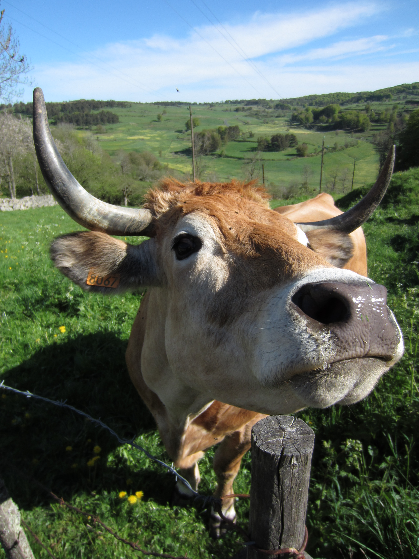
\includegraphics[height=6.5cm]{figures/speedup}
    \caption{Speedup}
    \label{figspeedup}
  \end{center}
\end{figure}

\begin{table}[h!]
  \begin{center}
    %\scriptsize{
    %\scalebox{0.89}{
    \begin{tabular}{>{\columncolor{lightgray}}c|ccc|ccc}
      \hline
      Length of the profiles &  \multicolumn{3}{c}{$20,000$} & \multicolumn{3}{c}{$100,000$} \\
      Number of profiles & 256 & 512 & 1024 & 256 & 512 & 1024\\
      \hline
      Average CPU time (min) & 10 & 10 & 10 & 10 & 10 & 10 \\
      \hline
    \end{tabular}
    %}
    \caption{Average performance of . on $48$ cores Opteron 2.2 GHz + memory}
    \label{tabtime}
  \end{center}
\end{table}
\bibliographystyle{plain}
\bibliography{biblio}


\end{document}
